\xchapter{Menções a software acadêmico de análise estática}
{Este capítulo apresenta uma revisão de literatura nas bases da ACM e IEEE em
busca de menções aos projetos de software acadêmico de análise estática
publicados nas conferências ASE e SCAM até o ano de 2015.}
\label{estudo2}

Este estudo caracterizou como os projetos de software acadêmico de análise
estática publicados nas conferências de Engenharia de Software ASE e SCAM são
mencionados em publicações nas bases ACM e IEEE.

A seção \ref{estudo2:introducao} contextualiza o estudo,
a seção \ref{estudo2:fundamentacao} apresenta os conceitos teóricos necessários para compreensão do trabalho,
a seção \ref{estudo2:definicao} descreve o objetivo e apresenta as questões de pesquisa,
a seção \ref{estudo2:planejamento} apresenta um planejamento do estudo,
as seções \ref{estudo2:preparacao} e \ref{estudo2:coleta} apresentam detalhes sobre a preparação e execução da coleta de dados,
as seções \ref{estudo2:analise} e \ref{estudo2:interpretacao} apresentam a análise e interpretação dos dados e
a seção \ref{estudo2:conclusoes} traça as conclusões finais deste estudo.

\section{Introdução e Motivação} \label{estudo2:introducao} % {{{

Os projetos de software desenvolvidos na academia sofrem de {\it
``dysfunctional chaotic churn''} \cite{howison2015understanding}.
Na prática, isso significa que há muitos projetos com características e
funcionalidades parecidas, com poucos usuários, com ciclos de vida curtos, e
encerrados quando o financiamento inicial termina, bem como, comunidades
desconectadas e paralelas, incompatibilidades entre projetos em um mesmo
domínio, e tentativas aparentemente não coordenadas de ``reiniciar'' tudo ({\it re-boots}). 

O desenvolvimento de sotware acadêmico é uma atividade que consome recursos
(tempo, dinheiro e atenção) e afeta a conduta da Ciência, tanto no geral como
em campos específicos, a colaboração no desenvolvimento destes projetos é uma
estratégia para lidar com a limitação dos baixos orçamentos das pesquisas, bem
como a limitação de tempo dos cientistas e a alta rotatividade entre os grupos
de pesquisa.

Especialmente em pesquisas na Engenharia de Software, onde, a princípio os
cientistas possuem o conhecimento necessário para colaboração, dessa forma,
neste estudo investigou-se como os projetos de software acadêmico de análise
estática publicados nas conferências ASE e SCAM até o ano de 2015 são vistos em
pesquisas nas bases da ACM e IEEE e quanta colaboração em relação ao
desenvolvimento e código fonte estes projetos recebem.

% }}}

\section{Fundamentação} \label{estudo2:fundamentacao} % {{{

\subsection{Menção}

Menção neste estudo refere-se a qualquer referência aos projetos de software
estudados, incluindo citações formais e informais, a prática científica de citação
formal amplamente adotada e praticada entre pesquisadores ainda não é realidade
entre artefatos digitais, a exemplo de projetos de software, que são citados
de maneiras variadas e distintas.

Software é citado na literatura acadêmica em notas de rodapé, em seções de
agradecimentos, ao longo do texto fazendo referência ao nome, ocasionalmente
encontra-se citações formais a projetos de software quando este possui
publicação associada.

Neste estudo as menções pesquisadas nas bases ACM e IEEE teve como critério
mínimo a identificação do projeto de software através do nome, ou seja, não
buscamos publicações que não fizessem menção ao nome do software.

% }}}

\section{Definição} \label{estudo2:definicao} % {{{

Quantas menções a projetos de software acadêmico de análise estática são
encontradas em publicações nas bases da ACM e IEEE? Como estes projetos são
mencionados? Existe contribuição em código fonte aos projetos?

\subsection{Definição do Objetivo}

\begin{description}
\item{\bf Objeto de estudo.} 
O objeto de estudo são projetos de software publicados nas conferências ASE e SCAM.

\item{\bf Propósito.} 
O propósito deste estudo é caracterizar menções aos projetos.

\item{\bf Perspectiva.} 
A perspectiva considerada é a de cientistas.

\item{\bf Foco de qualidade.} 
O principal aspecto de qualidade estudado é a visibilidade científica aos projetos.

\item{\bf Contexto.} 
O estudo foi conduzido com publicações das bases ACM e IEEE.
\end{description}

\subsection{Sumário da Definição}

Analisar os \textit{projetos de software acadêmico de análise estática publicados nas conferências ASE e SCAM}
com o propósito de \textit{caracterizar}
com respeito a \textit{visibilidade científica}
na perspectiva de \textit{cientistas}
no contexto de \textit{publicações nas bases ACM e IEEE}.

\subsection{Questões de Pesquisa}

Neste estudo as seguintes questões de pesquisa, a respeito dos projetos de
software acadêmico de análise estática, serão investigadas:

\newcommand{\EstudoDoisQuestaoUm}{Como os projetos de software acadêmico de
análise estática publicados nas conferências ASE e SCAM são mencionados em
publicações encontradas nas bases ACM e IEEE ao longo dos anos?}

\newcommand{\EstudoDoisQuestaoDois}{Os projetos de software acadêmico de
análise estática publicados nas conferências ASE e SCAM são utilizados,
caracterizados ou avaliados em estudos encontrados nas bases ACM e IEEE?}

\newcommand{\EstudoDoisQuestaoTres}{Os projetos de software acadêmico de
análise estática publicados nas conferências ASE e SCAM recebem contribuições
de código fonte em estudos encontrados nas bases ACM e IEEE?}

\begin{description}
  \item [Q1:] \EstudoDoisQuestaoUm
  \item [Q2:] \EstudoDoisQuestaoDois
  \item [Q3:] \EstudoDoisQuestaoTres
\end{description}

\subsection{Métricas}

Para responder às questões de pesquisas, as seguintes métricas serão usadas:

\begin{enumerate}
  \item Número de publicações nas bases ACM e IEEE mencionando projetos de
    software acadêmico de análise estática.
  \item Número de publicações nas bases ACM e IEEE mencionando uso,
    caracterização e avaliação a projetos de software acadêmico de análise
    estática.
  \item Número de publicações nas bases ACM e IEEE mencionando contribuição de
    código fonte aos projetos de software acadêmico de análise estática.
\end{enumerate}

% }}}

\section{Planejamento do Estudo} \label{estudo2:planejamento} % {{{

O estudo foi realizado a partir de uma revisão de literatura nas bases da ACM e
IEEE em busca de menções a projetos de software acadêmico de análise estática,
um esquema de classificação e caracterização de menções foi criado, os artigos
foram revisados segundo este esquema e as menções aos projetos foram coletadas
segundo esta classificação.

Este procedimento de revisão de literatura nas bases ACM e IEEE foi organizada
em quatro passos distintos -- Busca, Triagem, Keywording e Extração -- descritos
a seguir.

\subsection{Passo 1: Busca}

% strings de busca > conjunto de metadados bibtex

Este passo teve como objetivo principal encontrar artigos mencionando projetos
de software acadêmico de análise estática nas bases
ACM\footnote{\url{http://dl.acm.org}} e
IEEE\footnote{\url{http://ieeexplore.ieee.org}}, realizado manualmente através
da funcionalidade de busca avançada disponível publicamente no site de cada uma
dessas bases.

Na busca avançada no IEEE é necessário marcar a opção {\it Full Text \& Metadata}
para que a busca considere tanto os metadados quanto o conteúdo dos artigos, as Figuras
\ref{advanced-search-ieee} e \ref{advanced-search-acm} indicam quais campos
utilizados na busca avançada nestas bases.

\begin{figure}[h]
  \center
  \frame{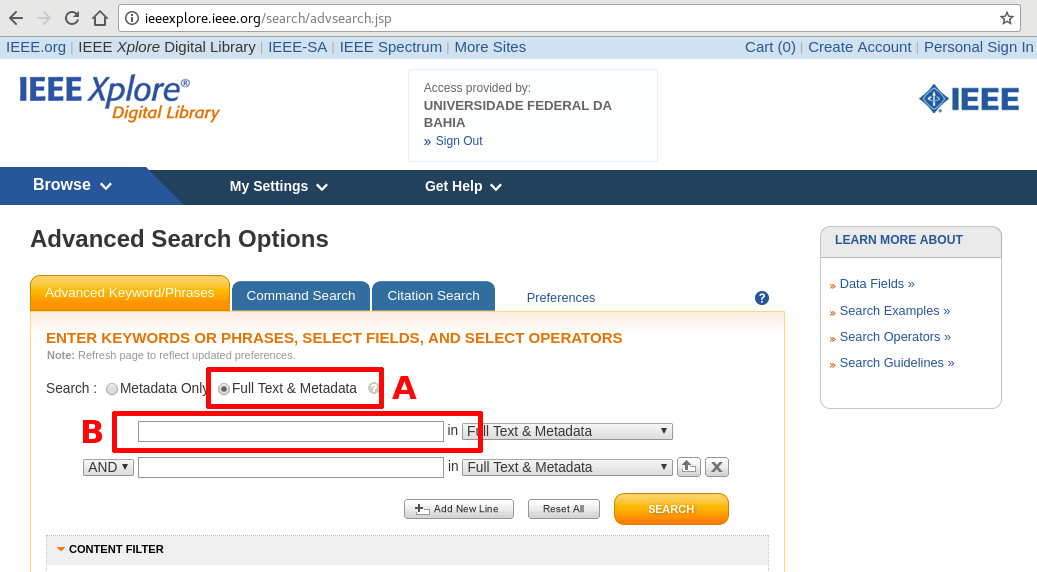
\includegraphics[scale=0.4]{imagens/advanced-search-ieee.png}}
  \caption{Captura de tela da busca avançada da base IEEE com destaque para a (A) opção de busca completa e para o (B) campo de entrada da string de busca.}
  \label{advanced-search-ieee}
\end{figure}

A busca avançada na base ACM (Figura \ref{advanced-search-acm}) não necessita
marcar nenhum campo adicional além do próprio campo texto onde deve-se entrar
com a string de busca de cada projeto. Para cada projeto de software são construídas duas strings, uma para busca na
base da ACM, outra para busca na base IEEE.

\begin{figure}[h]
  \center
  \frame{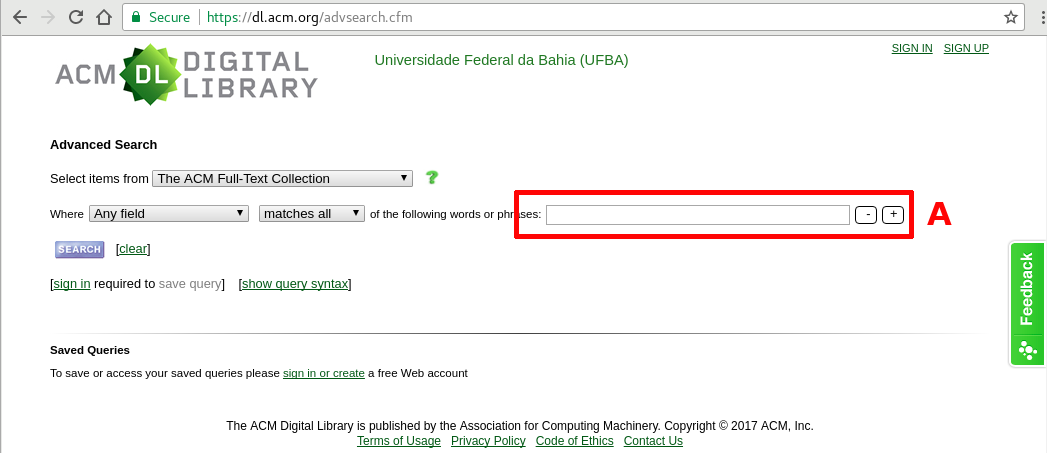
\includegraphics[scale=0.4]{imagens/advanced-search-acm.png}}
  \caption{Captura de tela da busca avançada da base ACM com destaque para o (A) campo de entrada da string de busca.}
  \label{advanced-search-acm}
\end{figure}

As strings de busca são elaboradas a partir dos dados coletados no estudo
anterior, como, nome do projeto, descrição, nome do autor da publicação
original, entre outros dados. A elaboração das strings é realizada num processo
incremental e iterativo, iniciando por uma busca utilizando apenas o nome do
projeto, avaliando os resultados, inspecionando o título de cada resultado,
refinando a string através de outras características do projeto quando os
resultados trazem muitos estudos sem relação com o projeto de software. Estas
strings são registradas no arquivo \texttt{search.yml} de cada projeto.

%buscamos inicialmente usando apenas o nome do software, analisamos o número total
%de resultados e os títulos destes resultados, quando o número de resultados for
%muito grande, acima de XXX, e os títulos não aparentavam ser estudos com relação
%aos projetos, incluímos mais características, como por exemplo, parte da descrição
%do software, ou parte da URL, autores, etc.

Os resultados trazidos pela string final são armazenados localmente em arquivos
no formato BibTeX, ambas as bases exportam os resultados neste formato, são
dois arquivos para cada projeto de software, um contendo os resultados da busca
na base ACM -- \texttt{acm.bib} -- e outro contendo os resultados da base IEEE
-- \texttt{ieee.bib}. O resultado final de todos estes arquivos serão
combinados e agregados num arquivo único sem duplicação de resultados contendo
os metadados de todos os artigos encontrados pelas strings de busca.

%
%, este arquivo contém os metadados de todos os
%artigos encontrados pelas strings de busca de cada projeto nas bases ACM e IEEE
%com um id único no formato \texttt{p + NUM}, exemplo \texttt{p1}, \texttt{p2},
%\texttt{p3}, etc.

Este arquivo único, localizado em \texttt{documents/references.bib},
além de eliminar as duplicidades de resultados, receberá também para
cada item uma identificação única, esta identificação será utilizada nas etapas
seguintes da revisão de literatura para relacionar os projeto com os
artigos através das menções identificadas.

%e pdf,
%estes resultados devem incluir ao menos os artigos selecionados
%no estudo anterior onde os projetos foram encontrados, já que tais artigos são
%o caso mínimo de resultado desejado nesta fase de busca. 

%de cada projeto, sem duplicidade, cada artigo receberá um ID único, este ID
%será utilizado nas etapas seguintes.

%, e um com um merge destes dois mantendo resultados únicos sem
%duplicidade.

%Para cada software, os resultados foram agrupados
%num arquivo único, sem duplicidade entre os resultados trazidos por cada base
%bibliográfica. O arquivo de metadados de cada software contém informações sobre
%o artigo, autores, ano de publicação, conferência, jornal, etc. Os artigos
%também foram armazenados localmente, no formato pdf para serem analisados na
%triagem.

\subsection{Passo 2: Triagem}

% leitura dos pdf > apenas os papers relevantes que mencionam o nome do software

Neste passo selecionamos os artigos relevantes para cada projeto entre os
resultados da busca avançada realizada para cada string, os artigos são
inspecionados manualmente em busca de confirmar se fazem realmente menção ao
projeto.

A primeira ação neste passo é fazer o download de cada artigo em formato pdf,
cada artigo presente no arquivo \texttt{documents/references.bib} será
inspecionado, os dados coletados neste passo serão armazenados no arquivo
\texttt{references.yml} de cada projeto, um campo chamado
\texttt{is\_software\_mentioned} deve ser criado com os valores \texttt{yes} ou
\texttt{no} indicando se o artigo menciona ou não o projeto.

A inspeção tem como objetivo selecionar os artigos relevantes para este estudo,
mantendo apenas aqueles com menção ao nome do software, seja a menção em
formato de citação formal ou informal.

%de cada artigo é realizada com o auxílio da funcionalidade de busca
%do leitor de pdf utilizado neste estudo\footnote{Utilizamos software Evince v3.22.1}
%utilizado para leitura dos artigos, com o auxílio da busca encontramos cada
%ocorrência ao nome do software tomando nota a confirmação sobre a menção
%encontrada.

%Esta informação foi armazenada no próprio arquivo BibTeX num campo adicional
%aos demais campos dos metadados do artigo; ao final, temos os metadados do
%artigo como, título, autores, ano de publicação, etc, e também uma indicação se
%o artigo cita realmente o software.

\subsection{Passo 3: Keywording}

% papers relevantes > esquema de tipos de menção

Neste passo será criado o esquema de codificação para classificação das
menções, o esquema é criado a partir da identificação do contexto em que os
projetos são mencionados, para cada menção toma-se nota no arquivo
\texttt{references.yml} no campo \texttt{review} sobre como o software é
mencionado naquele artigo.

As notas são comentários livres resumindo as menções encontradas no artigo
sobre um determinado software, um artigo científico pode mencionar um software
diversas vezes, de diversas formas, desde uma simples menção nos trabalhos
relacionados até uma grande contribuição ao software.

O conjunto final de todas as notas serão agrupadas e analisadas em conjunto com
o objetivo de criar um esquema de codificação para classificar as menções.
Este esquema deve ser construído como uma escala de pesos, onde o último tipo
de menção inclui implicitamente os tipos de menor peso, este peso representa
o nível de contribuição da menção ao ecossistema do projeto de software.

%Um tipo de menção com maior peso inclui implicitamente o tipo de menção de
%menor peso, e assim sucessivamente.

%, cada
%menção representa uma entrada em forma de contribução ao ecossistema, seja
%fazendo o projeto de software ser visível na literatura acadêmica, seja com
%contribuição direta em código ao projeto.

%Esta leitura irá gerar
%uma escala de tipos de menção ao software. Cada artigo assume, em relação ao
%software, um valor nesta escala de tipos de menção.

%Foi lido em busca de encontrar menções ao nome do software, em qual contexto o
%software é mencionado e de que forma é mencionado, resume cada tipo de menção com explicação dos casos em
%que se enquadram, o método utilizado para.

\subsection{Passo 4: Extração}

No último passo da revisão utiliza-se o esquema criado no passo anterior para
classificação das menções encontradas, para cada artigo será extraído qual o
tipo de menção é feito ao software, quando o artigo menciona o software
diversas vezes deve ser adotado o tipo de menção de maior relevância para este
estudo, onde o tipo de menção de maior peso inclui implicitamente os tipos
menores.

%A partir da classificação , Tabela \ref{esquema-de-mencao}, extraímos de cada
%artigo mencionando os projetos de acordo com o esquema de codificação criado no

Os dados extraídos são armazenados no arquivo \texttt{references.yml} de
cada projeto, sendo atualizado com a inclusão de um novo campo indicando o tipo
de menção do artigo ao software, \texttt{mention\_type}, este campo assume um dos
valores do esquema de classificação criado no passo anterior.

Ao final da revisão de literatura teremos para cada projeto de software um
conjunto de artigos com menções classificadas por tipo e contexto.

%, estando
%incluído nestes conjuntos ao menos os próprios artigos que deram origem ao
%conjunto de projetos utilizados como objeto de estudo neste trabalho.

%menções a eles nas bases do ACM e IEEE, temos o tipo de cada menção, se
%contribuiu com o projeto, se foi avaliado, ou apenas citado como referência, os
%artigos selecionados no estudo anterior que deram origem ao conjunto de
%projetos de software estão incluídos nestes resultados.

% }}}

\section{Preparação} \label{estudo2:preparacao} % {{{

Nesta seção apresentamos a preparação do estudo para a realização da coleta de
dados.

\subsection{Passo 1: Busca}

Seguindo o planejamento descrito em \ref{estudo2:planejamento}, criamos as
strings de busca para as bases ACM e IEEE de cada projeto. As strings foram
criadas buscando diretamente nessas duas bases e refinando os critérios quando
necessário. Foram registradas no arquivo \texttt{search.yml} de cada software,
além da própria string será registrado também o número de resultados e a data
em que a busca foi realizada.

%foram criados também campos para registrar o número de resultados da busca
%e a data em que a busca foi realizada registrada no formato UTC.

Segue abaixo a estrutura do arquivo \texttt{search.yml} com os campos para
armazenar os dados da busca, Listagem \ref{search-yml}.  Um documento
CSV com todas as strings de busca pode ser encontrado no repositório desta
dissertaçao no arquivo \texttt{documents/search-strings.csv}.

%Além do nome do software pesquisado, as strings de busca incluíram outras
%características do software sempre que necessário.

\begin{lstlisting}[
caption={Arquivo search.yml.},
label={search-yml},
frame=single,
numbers=left
]
  acm:
    string:
    searched_at:
    results:
  ieee:
    string:
    searched_at:
    results:
\end{lstlisting}

\subsection{Passo 2: Triagem}

Implementamos scripts para transformar os dados da busca em formato BibTeX para
arquivos no formato YML pois a coleta e inspeção dos artigos serão registrados
em arquivos YML para cada projeto de software. Estes scripts recebem como entrada
os resultados da busca de todos os projetos e geram como saída os arquivos \texttt{references.bib}
e \texttt{references.yml} para cada projeto.

\begin{description}

  \item[\texttt{bin/merge}]
    Agrega os arquivos \texttt{acm.bib}, \texttt{ieee.bib} e \texttt{paper.bib}
    de cada projeto em um único arquivo no formato BibTeX removendo
    duplicidades dos resultados.

  \item[\texttt{bin/ids}]
    Recebe a saída do script \texttt{bin/merge} e atribui a cada artigo um
    identificador único.

  \item[\texttt{bin/cache}]
    Cria um arquivo -- \texttt{cache/dataset.yml} -- no formato YAML agregando todos os dados coletados de todos
    os projetos a partir dos arquivos \texttt{software.yml}, \texttt{acm.bib},
    \texttt{ieee.bib}, \texttt{paper.bib}, \texttt{references.yml} e
    \texttt{search.yml}.

  \item[\texttt{bin/render}]
    Lê o arquivo de cache, carrega os dados em memória e passa estes dados como
    parâmetro para os arquivos templates.

\end{description}

Todos estes scripts estão disponíveis no repositório desta dissertação e foram desenvolvidos
utilizando a a linguagem de
programação Perl\footnote{\url{http://perl.org}} com o auxílio dos
módulos CPAN: Modern::Perl\footnote{\url{http://metacpan.org/pod/Modern::Perl}},
YAML\footnote{\url{http://metacpan.org/pod/YAML}},
Mojo::Template\footnote{\url{http://metacpan.org/pod/Mojo::Template}},
Text::BibTeX\footnote{\url{http://metacpan.org/pod/Text::BibTeX}} e
List::Util\footnote{\url{http://metacpan.org/pod/List::Util}}.

A maior parte da lógica destes scripts foram implementadas no arquivo
\texttt{lib/Dissertacao.pm} com objetivo de reduzir repetição de código e
proporcionar reuso. O fluxo de informações entre estes scripts e os arquivos
utilizados como entrada e saída estão representados em resumo no fluxograma da
Figura \ref{estudo2-fluxograma}.

\begin{figure}[h]
  \center
  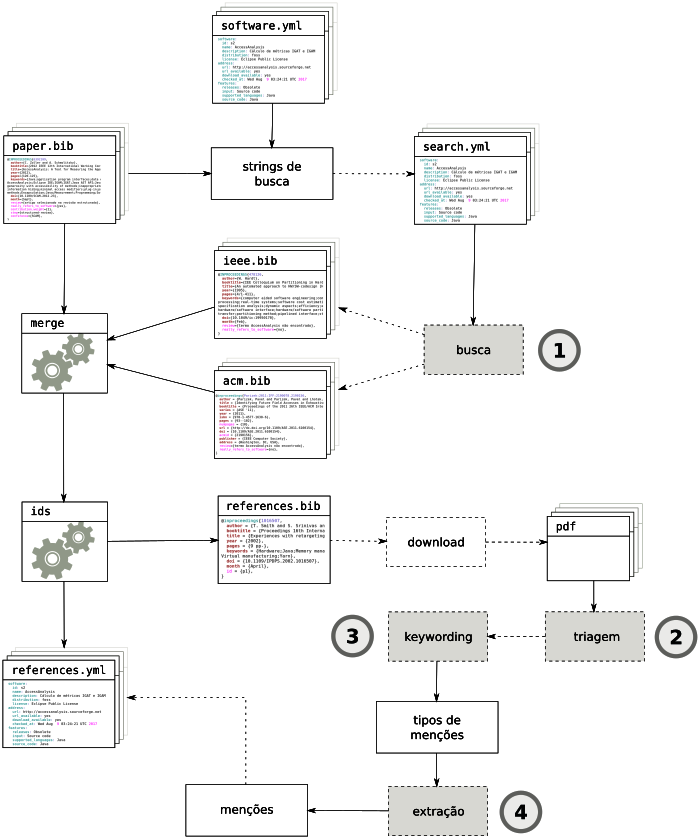
\includegraphics[scale=0.35]{imagens/estudo2-fluxograma.png}
  \caption{Fluxo de coleta, análise e transformação dos dados.}
  \label{estudo2-fluxograma}
\end{figure}

%Definimos uma identificação única para cada um dos 60 projetos de software
%utilizando o próprio arquivo \texttt{software.yml} através do campo
%\texttt{id:} seguindo o padrão \texttt{s + número}, exemplo, \texttt{s1},
%\texttt{s2}, \texttt{s3}, \texttt{s4}, ..., \texttt{s60}, cada projeto de software
%recebeu um id.

%Definimos um novo campo neste mesmo arquivo para coleta das menções, fazendo
%referência ao ID do artigo mencionando o software, com os campos ... cada artigo
%encontrado na revisão de literatura também receberá um ID, desta forma será possível
%relacionar projetos e artigos através das menções.
%
%...

\subsection{Passo 3: Keywording}

Preparamos o template para criar os arquivos inicials \texttt{references.yml}
para cada projeto, a Listagem \ref{references-yml} apresenta um exemplo do
trecho do YML para armazenar a extração dessas informações.

\begin{lstlisting}[
caption={Arquivo references.yml.},
label={references-yml},
frame=single,
numbers=left
]
  p1:
    review:
    is_software_mentioned:
  p2:
    review:
    is_software_mentioned:
  p3:
    review:
    is_software_mentioned:
\end{lstlisting}

\subsection{Passo 4: Extração}

Criamos os templates para representação dos dados coletados em formato CSV
para utilizar na etapa de análise. Implementamos também templates para gerar arquivos em
formato TeX para posterior inclusão na seção de coleta onde apresentaremos os dados
coletados.

%Os dados armazenados em arquivos
%YAML e BibTeX são carregados em estruturas em memória através de um script
%escrito em linguagem Perl e repassados para templates processados para exibir
%os dados neste texto, em arquivos TeX, CSV, etc. A Figura \ref{estudo2-fluxograma}
%apresenta o fluxo de coleta, análise e transformação dos dados.

% }}}

\section{Coleta de dados} \label{estudo2:coleta} % {{{

Seguindo o planejamento e preparação descritos nas seções
\ref{estudo2:planejamento} e \ref{estudo2:preparacao} iniciamos a coleta dos
dados através de uma revisão de literatura nas bases ACM e IEEE.

% dados do estudo1
\newcommand{\SoftwareCount}{60}
\newcommand{\SoftwareUrlNotAvailableCount}{15}
\newcommand{\SoftwareUrlAvailableCount}{45}
\newcommand{\SoftwareDownloadNotAvailableCount}{24}
\newcommand{\SoftwareDownloadAvailableCount}{36}
% dados do estudo2
\newcommand{\SearchACMCount}{438}
\newcommand{\SearchIEEECount}{459}
\newcommand{\SearchCount}{897}
\newcommand{\SearchUniqueCount}{806}
\newcommand{\ScreeningCount}{429}
\newcommand{\ScreeningUniqueCount}{416}
\newcommand{\CiteCount}{199}
\newcommand{\UseCount}{124}
\newcommand{\ContributeCount}{106}
\newcommand{\SearchUniqueMean}{13.4}
\newcommand{\ScreeningMean}{7.2}
\newcommand{\ScreeningUniqueMean}{6.9}
\newcommand{\MentionsStudyUm}{60}
\newcommand{\MentionsStudyDois}{47}
\newcommand{\SoftwareNotMentionedCount}{13}
\newcommand{\ContributeStudyDoisCount}{43}
\newcommand{\ContributeStudyDoisSoftware}{17}
% dados do estudo3
\newcommand{\ReleasesCount}{303}
\newcommand{\ReleasesAvailableCount}{211}
\newcommand{\ReleasesMetricsCount}{206}
\newcommand{\ProjectsWithReleasesCount}{35}
\newcommand{\ProjectsAnalizedCount}{24}
\newcommand{\ReleasesYearFirst}{2001}
\newcommand{\ReleasesYearLast}{2017}


\subsection{Passo 1: Busca}

As strings de busca foram definidas e a busca nas bases foi realizada para cada
software acadêmico do conjunto, encontramos um total de \SearchCount \
resultados ao somar o número de resultados de cada software nas bases ACM e
IEEE, deste total, \SearchACMCount \ foi encontrado na base ACM e
\SearchIEEECount \ foi encontrado na base IEEE.

Este resultado total inclui duplicação entre as buscas dos projetos, ou seja,
um mesmo artigo foi encontrado nas duas bases, e também um mesmo artigo foi
encontrado em busca de projetos distintos, dentre o resultado total,
\SearchUniqueCount \ são únicos, ou seja, encontramos \SearchUniqueCount \ artigos.

A lista completa com autores, título e ano de publicação com todos os
\SearchUniqueCount \ resultados pode ser consultado no arquivo
\texttt{documents/search.md} no repositório desta dissertação.

%Alguns artigos fazem menção a mais de 1 projeto, fizemos o download de cada
%artigo e armazenamos os metadados em formato BibTeX nos arquivos \texttt{acm.bib}
%e \texttt{ieee.bib} para cada projeto de software.

Na sequencia adicionamos o \texttt{id} a cada artigo do
\texttt{documents/references.bib}, este arquivo tem os metadados dos artigos
encontrados, eles receberam ids, estes ids serão
utilizados para relacionar o projeto ao artigo, o script \texttt{bin/ids}
foi utilizado para automatizar esta função.

A Tabela \ref{search-table} ...

\begin{longtable}{ l c c c | l c c c }
\caption{Número de resultados obtidos na busca de cada projeto de software.}
\label{search-table} \\
  \hline
  \hhline{ l c c c | l c c c |}
  \endfirsthead
  \hhline{ l c c c | l c c c |}
  \hline
   \multirow{2}{*}{\textbf{ID}} & \multicolumn{2}{c}{{\bf Busca}} & \multirow{2}{*}{\textbf{Total}} & \multirow{2}{*}{\textbf{ID}} & \multicolumn{2}{c}{{\bf Busca}} & \multirow{2}{*}{\textbf{Total}} \\
   & \textbf{ACM} & \textbf{IEEE} & & & \textbf{ACM} & \textbf{IEEE} & \\
  \hline
  \hhline{ l c c c | l c c c |}
  \endhead
  \hhline{----|----}
  \multicolumn{8}{c}{continua na próxima página} \\
  \hhline{----|----} \endfoot
  \hhline{----|----} \endlastfoot
   \multirow{2}{*}{\textbf{ID}} & \multicolumn{2}{c}{{\bf Busca}} & \multirow{2}{*}{\textbf{Total}} & \multirow{2}{*}{\textbf{ID}} & \multicolumn{2}{c}{{\bf Busca}} & \multirow{2}{*}{\textbf{Total}} \\
   & \textbf{ACM} & \textbf{IEEE} & & & \textbf{ACM} & \textbf{IEEE} & \\
  \hline
\texttt{s1} & 11 & 26 & 38 & \texttt{s32} & 19 & 18 & 32 \\
\texttt{s2} & 5 & 3 & 8 & \texttt{s33} & 3 & 3 & 5 \\
\texttt{s3} & 10 & 6 & 15 & \texttt{s34} & 1 & 3 & 4 \\
\texttt{s4} & 4 & 6 & 9 & \texttt{s35} & 2 & 1 & 2 \\
\texttt{s5} & 4 & 3 & 6 & \texttt{s36} & 17 & 20 & 34 \\
\texttt{s6} & 6 & 2 & 7 & \texttt{s37} & 2 & 5 & 7 \\
\texttt{s7} & 16 & 9 & 25 & \texttt{s38} & 29 & 20 & 42 \\
\texttt{s8} & 7 & 7 & 13 & \texttt{s39} & 3 & 10 & 11 \\
\texttt{s9} & 4 & 4 & 8 & \texttt{s40} & 3 & 8 & 11 \\
\texttt{s10} & 12 & 4 & 14 & \texttt{s41} & - & - & 1 \\
\texttt{s11} & 2 & 2 & 3 & \texttt{s42} & 1 & 4 & 5 \\
\texttt{s12} & 6 & 1 & 6 & \texttt{s43} & - & 2 & 2 \\
\texttt{s13} & 6 & 3 & 9 & \texttt{s44} & 3 & 1 & 3 \\
\texttt{s14} & 1 & 1 & 2 & \texttt{s45} & 5 & 10 & 14 \\
\texttt{s15} & 15 & 4 & 16 & \texttt{s46} & 16 & 12 & 24 \\
\texttt{s17} & - & 1 & 1 & \texttt{s47} & 6 & 7 & 13 \\
\texttt{s16} & 1 & 4 & 5 & \texttt{s48} & 3 & 2 & 4 \\
\texttt{s18} & 23 & 24 & 47 & \texttt{s49} & 1 & 4 & 5 \\
\texttt{s19} & 20 & 30 & 45 & \texttt{s50} & 1 & 1 & 2 \\
\texttt{s20} & 7 & 3 & 10 & \texttt{s51} & 2 & 5 & 7 \\
\texttt{s21} & 1 & 3 & 3 & \texttt{s52} & 9 & 34 & 41 \\
\texttt{s22} & 4 & 4 & 5 & \texttt{s53} & 10 & 5 & 13 \\
\texttt{s23} & 2 & 11 & 12 & \texttt{s54} & 2 & 2 & 4 \\
\texttt{s24} & - & - & 1 & \texttt{s55} & 3 & 8 & 12 \\
\texttt{s25} & 20 & 17 & 34 & \texttt{s56} & 23 & 21 & 38 \\
\texttt{s26} & 5 & 2 & 7 & \texttt{s57} & 4 & 6 & 8 \\
\texttt{s27} & 2 & 4 & 5 & \texttt{s58} & 8 & 4 & 11 \\
\texttt{s28} & 26 & 24 & 50 & \texttt{s59} & 25 & 12 & 36 \\
\texttt{s29} & 11 & 5 & 15 & \texttt{s60} & - & 7 & 7 \\
\texttt{s30} & 4 & 9 & 10 & \texttt{{\bf Média}} & {\bf 7.3} & {\bf 7.7} & {\bf 13.8} \\
\texttt{s31} & 2 & 2 & 3 & \texttt{{\bf Total}} & {\bf 438} & {\bf 459} & {\bf 830} \\
\end{longtable}


%Os scripts \texttt{bin/merge},  foram utilizados para gerar o
%\texttt{documents/references.bib} a partir dos arquivos \texttt{acm.bib},
%\texttt{ieee.bib} e \texttt{paper.bib} de cada projeto.

\subsection{Passo 2: Triagem}

Os \SearchUniqueCount \ artigos foram inspecionados em busca de menções aos
projetos de software, para cada projeto foi analisado o conjunto de artigos
retornado pela string de busca daquele projeto. O critério da inspeção considerou qualquer ocorrencia ao nome do projeto de
software nos artigos do conjunto da busca do projeto, alguns projetos de
software possui nomes comuns que foram encontrados nos artigos mas não faziam
referencia ao software, em alguns casos os nomes apareciam em fórmulas
matemáticas ou como parte de um outra palavra.

Ao final da triagem foi selecionado para cada um dos \SoftwareCount \ projetos um conjunto de artigos
que de fato mencionam o software, ainda sem caracterizar o tipo de menção,
apenas se realmente menciona, ao total selecionamos \ScreeningCount \ menções.
Este total de menções foram encontrados ao meio a \ScreeningUniqueCount \
artigos.

Uma tabela no formato CSV com todos os artigos e projetos, indicando quando há
relação entre eles através de menção pode ser encontrada no repositório desta
dissertação no arquivo \texttt{documents/references.csv}, neste arquivo todos
os artigos e todos os projetos são representados e a relação entre eles é
marcada com um \texttt{x} sempre que houver menção de um artigo para um
software.

%Merge único de todos os arquivos BibTeX, incluindo o arquivo \texttt{paper.bib} de
%cada projeto gerado no estudo anterior apresentado no Capítulo \ref{estudo1}, um
%arquivo \texttt{documents/references.bib} foi criado contendo todas as referências
%a todos os projetos, referências únicas.

%334 artigos fazem menção aos 60 projetos.
%350 não faz menção aos projetos.

\subsection{Passo 3: Keywording}

A avaliação das \ScreeningCount \ menções gerou uma escala de tipos de menção
aos projetos de software, detalhado na Tabela \ref{esquema-de-mencao}, com três valores
distintos, onde o último tipo de menção com maior valor inclui todos os demais.

\begin{table}[h]
\caption{Esquema para classificação de menções aos projetos software acadêmico.}
\centering
\begin{tabular}{ l p{10cm} }
  \hline
  Tipo de menção           & Explicação \\
  \hline
  Cita      & Apenas cita o software ou é o mesmo artigo onde o software selecionado; É um artigo com ``mesmo'' conteúdo publicado na ``mesma'' época; O artigo apenas descreve o software; Menciona o software numa tabela com outros, classifica; Menciona o software como exemplo; Menciona o software como trabalho relacionado; Menciona o software em trabalhos futuros. \\
  Usa       & Avalia ou caracteriza o software; Usa para coleta ou análise de dados; Usa como objeto de estudo; Usa o software como parte de uma solução, implementação, etc; Cria um software derivado mas não disponibiliza as contribuições. \\
  Contribui & Cria; Contribuição inicial criando o projeto; Faz uma grande contribuição; Refatora todo o software; Abre o código de um software que antes era de código fechado; Contribuição pequena ou moderada; Extende o software; Integra o software a outros sistemas, formatos de entrada/saída, APIs, etc; Refatora parte do software; Implementa parte do software em outro projeto e compara resultados. \\
  \hline
\end{tabular}
\label{esquema-de-mencao}
\end{table}

A definição deste esquema foi feito através de anotações sobre onde e como o
projeto de software é mencionado em cada artigo, anotamos no campo
\texttt{review} do arquivo \texttt{references.yml} um comentário textual livre
resumindo de que forma o projeto de software é mencionado, caso várias menções
seja encontrado num mesmo artigo para um dado projeto de software é feito um
resumo total.

%Esta anotação foi feita no arquivo \texttt{references.yml} de cada projeto, nele
%foi adicionado um novo registro para cada artigo que faz menção e notas sobre a
%menção foi adicionada.

É importante lembrar que um mesmo artigo pode mencionar
mais de um software.

%também o tipo de menção que é feita ao software: se apenas cita como exemplo,
%se contribui com novos algoritmos e técnicas, se avalia, ou apenas descreve o
%software comparando-o com outro software.

\subsection{Passo 4: Extração}

%Coletamos as informações relacionadas a cada menção encontrada, cada um dos
%\ScreeningUniqueCount \ artigos encontrados mencionando os projetos, coletamos
%como o projeto é mencionado, encontramos \ScreeningCount \ menções aos
%projetos neste conjunto de artigos.

A partir do esquema para caracterização das menções coletamos os valores para o
campo \texttt{mention\_type} assumindo um dos valores da Tabela
\ref{esquema-de-mencao}: \texttt{cite} (Cita), \texttt{use} (Usa) ou
\texttt{contribute} (Contribui). Encontramos \CiteCount \ menções do tipo Cita,
\UseCount \ menções do tipo Usa e
\ContributeCount \ menções do tipo Contribui.

Os dados coletados na revisão de literatura durante os quatro passos são
apresentados em resumo na Tabela \ref{mentions-table} indicando o
número de resultados encontrados para cada projeto de software.

\begin{longtable}{ l c c c c | l c c c c }
\caption{Número de menções por tipo para cada projeto.}
\label{mentions-table} \\
  \hline
  \hhline{ l c c c c | l c c c c |}
  \endfirsthead
  \hhline{ l c c c c | l c c c c |}
  \hline
   \multirow{2}{*}{\textbf{ID}} & \multicolumn{3}{c}{{\bf Menções}} & \multirow{2}{*}{\textbf{Total}} & \multirow{2}{*}{\textbf{ID}} & \multicolumn{3}{c}{{\bf Menções}} & \multirow{2}{*}{\textbf{Total}} \\
   & \textbf{Cita} & \textbf{Usa} & \textbf{Contribui} & & & \textbf{Cita} & \textbf{Usa} & \textbf{Contribui} & \\
  \hline
  \hhline{ l c c c c | l c c c c |}
  \endhead
  \hhline{-----|-----}
  \multicolumn{10}{c}{continua na próxima página} \\
  \hhline{-----|-----} \endfoot
  \hhline{-----|-----} \endlastfoot
   \multirow{2}{*}{\textbf{ID}} & \multicolumn{3}{c}{{\bf Menções}} & \multirow{2}{*}{\textbf{Total}} & \multirow{2}{*}{\textbf{ID}} & \multicolumn{3}{c}{{\bf Menções}} & \multirow{2}{*}{\textbf{Total}} \\
   & \textbf{Cita} & \textbf{Usa} & \textbf{Contribui} & & & \textbf{Cita} & \textbf{Usa} & \textbf{Contribui} & \\
  \hline
\texttt{s1} & - & - & 1 & 1 & \texttt{s32} & 8 & - & 6 & 14 \\
\texttt{s2} & 1 & - & 1 & 2 & \texttt{s33} & 2 & 2 & 1 & 5 \\
\texttt{s3} & 3 & - & 1 & 4 & \texttt{s34} & 1 & - & 1 & 2 \\
\texttt{s4} & 4 & 3 & 2 & 9 & \texttt{s35} & - & - & 1 & 1 \\
\texttt{s5} & 2 & - & 3 & 5 & \texttt{s36} & 1 & - & 1 & 2 \\
\texttt{s6} & 4 & - & 1 & 5 & \texttt{s37} & 3 & 1 & 3 & 7 \\
\texttt{s7} & 9 & - & 1 & 10 & \texttt{s38} & 17 & - & 1 & 18 \\
\texttt{s8} & 3 & 1 & 2 & 6 & \texttt{s39} & 1 & - & 1 & 2 \\
\texttt{s9} & - & - & 5 & 5 & \texttt{s40} & 1 & 5 & 3 & 9 \\
\texttt{s10} & 1 & 2 & 2 & 5 & \texttt{s41} & - & - & 1 & 1 \\
\texttt{s11} & 2 & - & 1 & 3 & \texttt{s42} & - & - & 1 & 1 \\
\texttt{s12} & 1 & - & 1 & 2 & \texttt{s43} & - & - & 2 & 2 \\
\texttt{s13} & - & - & 1 & 1 & \texttt{s44} & 1 & - & 1 & 2 \\
\texttt{s14} & 1 & - & 1 & 2 & \texttt{s45} & - & - & 2 & 2 \\
\texttt{s15} & 4 & - & 1 & 5 & \texttt{s46} & 9 & 3 & 1 & 13 \\
\texttt{s17} & - & - & 1 & 1 & \texttt{s47} & - & - & 1 & 1 \\
\texttt{s16} & 1 & 1 & 2 & 4 & \texttt{s48} & 1 & - & 1 & 2 \\
\texttt{s18} & - & 1 & 1 & 2 & \texttt{s49} & 1 & 2 & 2 & 5 \\
\texttt{s19} & 14 & 18 & 8 & 40 & \texttt{s50} & - & - & 1 & 1 \\
\texttt{s20} & - & - & 1 & 1 & \texttt{s51} & 1 & 2 & 1 & 4 \\
\texttt{s21} & - & - & 1 & 1 & \texttt{s52} & 14 & 23 & 3 & 40 \\
\texttt{s22} & 2 & - & 1 & 3 & \texttt{s53} & 1 & 2 & 1 & 4 \\
\texttt{s23} & 3 & 2 & 3 & 8 & \texttt{s54} & 1 & 1 & 1 & 3 \\
\texttt{s24} & - & - & 1 & 1 & \texttt{s55} & - & - & 1 & 1 \\
\texttt{s25} & 5 & 10 & 4 & 19 & \texttt{s56} & 15 & 5 & 1 & 21 \\
\texttt{s26} & 3 & 2 & 2 & 7 & \texttt{s57} & 4 & - & 1 & 5 \\
\texttt{s27} & - & 2 & 1 & 3 & \texttt{s58} & 5 & 5 & 1 & 11 \\
\texttt{s28} & 22 & 14 & 4 & 40 & \texttt{s59} & 16 & 10 & 7 & 33 \\
\texttt{s29} & 5 & 1 & 1 & 7 & \texttt{s60} & 4 & - & 1 & 5 \\
\texttt{s30} & 2 & 5 & 1 & 8 & \texttt{{\bf Média}} & {\bf 3.3} & {\bf 2.1} & {\bf 1.8} & {\bf 7.2} \\
\texttt{s31} & - & 1 & 1 & 2 & \texttt{{\bf Total}} & {\bf 199} & {\bf 124} & {\bf 106} & {\bf 429} \\
\end{longtable}


% }}}

% Raw results from the analysis
\section{Análise dos Dados} \label{estudo2:analise} % {{{

Dados de 60 projetos de software acadêmico de análise estática desenvolvidos e
publicados na literatura acadêmica de engenharia de software, informações sobre
diversas formas de menção ao nome destes projetos na literatura acadêmica nas
bases ACM e IEEE entre \SearchUniqueCount \ artigos distintos.
%o número de autores mencionando o software ao longo do tempo.

\subsection{Passo 1: Busca}

Dentre todos os projetos dois não encontrou nenhuma ocorrência na busca --
\texttt{s24} (GUIZMO) e \texttt{s41} (protopurity) -- as strings de busca
destes dois projetos não encontrou nenhum resultado, tanto na base ACM quanto
na base IEEE.

A média de resultados por projeto foi de \SearchUniqueMean \ artigos. Entre os
projetos com maior número de resultados (acima da média) a maioria está entre
os projetos disponível para download, 11 com acesso e 7 sem acesso.
Entre os projetos com número de resultados abaixo da média 25 estão entre os
projetos com acesso a download e 16 sem acesso a download.

%projetos com resultado da busca acima da média
% resultados  acesso
% s1  38      s
% s3  15      n
% s7  25      s
% s10 14      s
% s15 16      n
% s18 47      s
% s19 45      n
% s25 34      s
% s28 50      s
% s29 15      s
% s32 32      s
% s36 34      n
% s38 42      n
% s45 14      n
% s46 24      s
% s52 41      s
% s56 38      n
% s59 36      s
% s = 11
% n = 7

%projetos com resultado da busca abaixo da média
%resultados acesso
%s2  8      s
%s4  9      n
%s5  6      n
%s6  7      s
%s8  13     s
%s9  8      n
%s11 3      n
%s12 6      s
%s13 9      n
%s14 2      s
%s16 5      s
%s17 1      s
%s20 10     n
%s21 3      s
%s22 5      s
%s23 12     n
%s24 1      s
%s26 7      s
%s27 5      s
%s30 10     n
%s31 3      n
%s33 5      s
%s34 4      s
%s35 2      s
%s37 7      s
%s39 11     n
%s40 11     s
%s41 1      s
%s42 5      s
%s43 2      s
%s44 3      n
%s48 4      n
%s49 5      n
%s50 2      s
%s51 7      s
%s53 13     n
%s54 4      s
%s55 12     s
%s57 8      n
%s58 11     s
%s60 7      n

\subsection{Passo 2: Triagem}

Total de \ScreeningCount \ menções, média de \ScreeningMean \ menções por
projeto.  Entre os projetos com menções acima da média total, 9 com acesso a
download e 6 sem acesso a download, entre os projetos com menções abaixo da
média, 25 com acesso, 20 sem acesso.

% acima da média de menções
%          acesso
%s4  = 9   n
%s7  = 10  s
%s19 = 40  n
%s23 = 8   n
%s25 = 19  s
%s28 = 40  s
%s30 = 8   n
%s32 = 14  s
%s38 = 18  n
%s40 = 9   s
%s46 = 13  s
%s52 = 40  s
%s56 = 21  n
%s58 = 11  s
%s59 = 33  s

% abaixo da média de menções
%         acesso
%s1  = 1  s
%s2  = 2  s
%s3  = 4  n
%s5  = 5  n
%s6  = 5  s
%s8  = 6  s
%s9  = 5  n
%s10 = 5  s
%s11 = 3  n
%s12 = 2  s
%s13 = 1  n
%s14 = 2  s
%s15 = 5  n
%s16 = 4  n
%s17 = 1  s
%s18 = 2  s
%s20 = 1  n
%s21 = 1  s
%s22 = 3  s
%s24 = 1  s
%s26 = 7  s
%s27 = 3  s
%s29 = 7  s
%s31 = 2  n
%s33 = 5  s
%s34 = 2  s
%s35 = 1  s
%s36 = 2  n
%s37 = 7  s
%s39 = 2  n
%s41 = 1  s
%s43 = 2  s
%s44 = 2  n
%s45 = 2  n
%s47 = 1  n
%s48 = 2  n
%s49 = 5  n
%s50 = 1  s
%s51 = 4  s
%s53 = 4  n
%s54 = 3  s
%s55 = 1  s
%s57 = 5  n
%s60 = 5  n

\subsection{Passo 3: Keywording}

\CiteCount \ Cita,
\UseCount \ Usa e
\ContributeCount \ Contribui.

\subsection{Passo 4: Extração}

Entre os \SoftwareCount \ projetos de software estudados
\SoftwareNotMentionedCount \ não foram encontrados na revisão de literatura em
publicações após a publicação inicial
(\texttt{s1}, \texttt{s13}, \texttt{s17}, \texttt{s20}, \texttt{s21}, \texttt{s24}, \texttt{s35}, \texttt{s41}, \texttt{s42}, \texttt{s43}, \texttt{s47}, \texttt{s50}, \texttt{s55}, \texttt{s61}, \texttt{s62}, \texttt{s63}, \texttt{s65}, \texttt{s66}, \texttt{s68}
), tendo apenas a publicação
inicial onde o software foi selecionado no estudo apresentado no Capítulo
\ref{estudo1}.

%cada um, alguns tendo duas publicações na mesma época sendo uma
%publicação específica numa trilha de ferramenta, ou senndo 2 artigos
%semelhantes publicados na mesma época em conferências distintas, mas sendo os
%mesmos autores.

%Nenhum destes projetos tiveram menção após a publicação inicial do projeto,
%entre estes 14 projetos, apenas três (Diagnosys, ETXL e Rêve) estão
%indisponíveis para download, os outros 11 estão disponíveis, todos com código
%fonte, exceto o FaultBuster que está disponível apenas em formato binário.

Entre os \MentionsStudyDois \
projetos mencionados após a publicação inicial encontrada na literatura.
A Figura \ref{mentions-timeline} apresenta uma visualização da linha do tempo
de cada software em relação a menções encontradas nas bases ACM e IEEE através
da revisão de literatura.

\begin{figure}[h]
  \center
  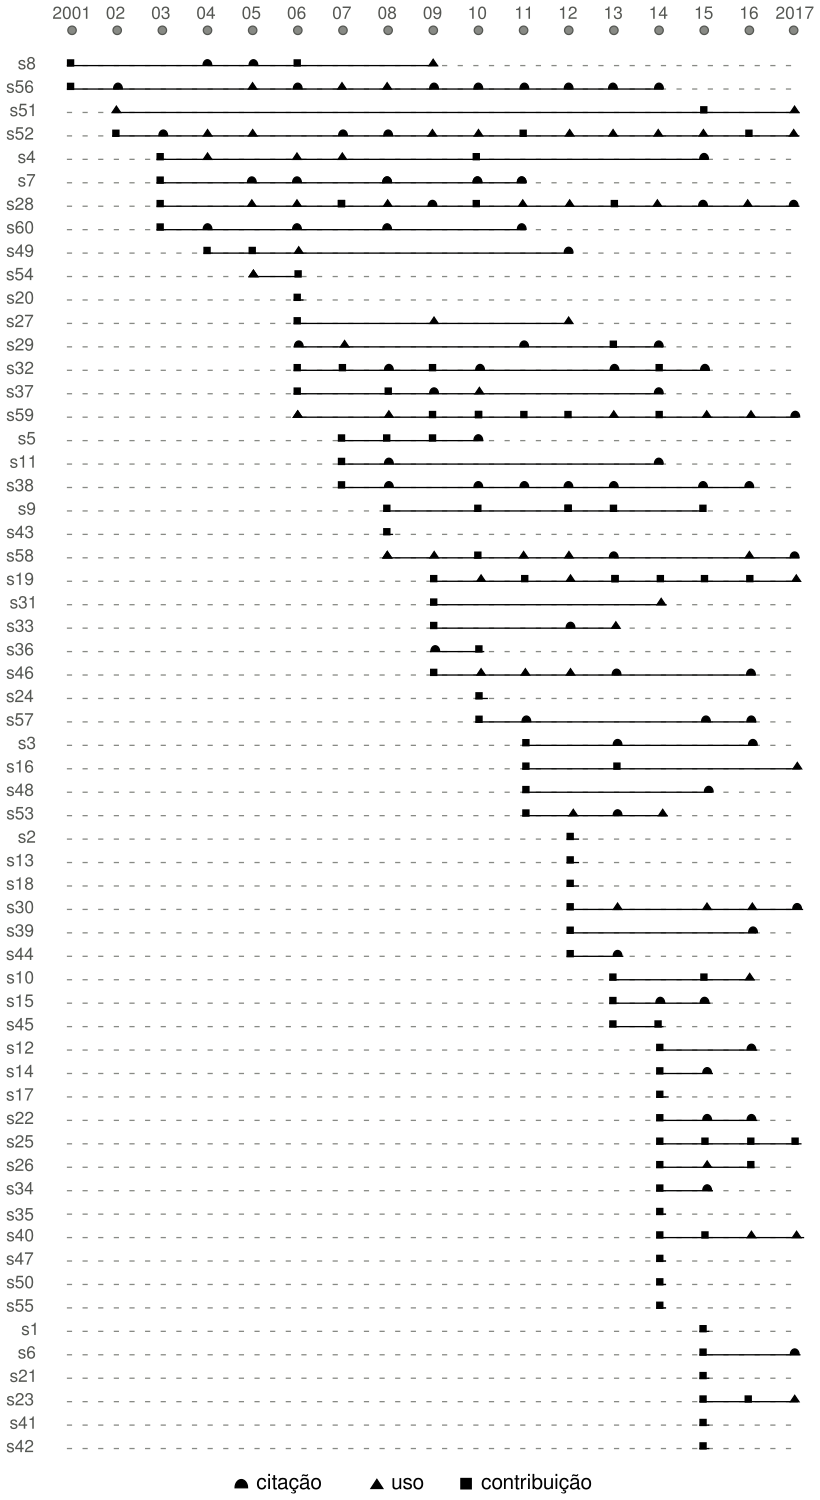
\includegraphics[scale=0.6]{imagens/mentions-timeline.png}
  \caption{Linha do tempo de menções (uso e contribuição) aos projetos nas bases ACM e IEEE.}
  \label{mentions-timeline}
\end{figure}

%Ao todo foram encontradas 465 menções aos 60 projetos de software, estas
%menções estão num conjunto de 334 artigos selecionados na revisão de literatura
%nas bases ACM e IEEE.

%Entre todas as menções a maior parte (222) apenas cita os projetos de software
%como exemplo de implementação, apenas cita o software ou é o mesmo artigo onde
%o software selecionado; É um artigo com “mesmo” conteúdo publicado na “mesma”
%época; O artigo apenas descreve o software; Menciona o software numa tabela com
%outros, classifica; Menciona o software como exemplo; Menciona o software como
%trabalho relacionado; Menciona o software em trabalhos futuros.

% ./bin/mentions dataset/software/*/references.bib contribution_weight=0.1 | grep " title = " | wc -l
%AS 222 menções foram encontradas em 204 artigos distintos.

\ContributeStudyDoisCount \ menções com contribuição a
\ContributeStudyDoisSoftware \ projetos de software
(\texttt{s10}, \texttt{s19}, \texttt{s23}, \texttt{s25}, \texttt{s26}, \texttt{s28}, \texttt{s32}, \texttt{s37}, \texttt{s4}, \texttt{s40}, \texttt{s45}, \texttt{s49}, \texttt{s5}, \texttt{s52}, \texttt{s59}, \texttt{s67}, \texttt{s8}, \texttt{s9}
).

% }}}

% Hypothesis rejection
\section{Interpretação dos Resultados} \label{estudo2:interpretacao} % {{{

\subsection{Q1 - \EstudoDoisQuestaoUm}

% Demográfica.

\subsection{Q2 - \EstudoDoisQuestaoDois}

Entre as 465 menções encontradas, 130 são menções que avalia ou caracteriza o
software; Usa para coleta ou análise de dados; Usa como objeto de estudo; Usa o
software como parte de uma solução, implementação, etc; Cria um software
derivado mas não disponibiliza as contribuições.

Entre os 60 projetos de software, 27 são mencionados entre estas 130 menções
encontradas.

% ./bin/mentions dataset/software/*/references.bib contribution_weight=0.25

Entre as 130 menções, foram encontradas entre 125 artigos distintos.

\subsection{Q3 - \EstudoDoisQuestaoTres}

Número de menções a cada software acadêmico e qual o contexto e tipo de menção
é feita, quem e quantos são os autores de cada menção.

% ./bin/mentions dataset/software/*/references.bib contribution_weight=0.5

40 menções contribuindo com os projetos foram encontrados, cada menção
encontrado num artigo distinto. Estas 40 menções são em relação a apenas
16 projetos entre os 60 do conjunto total, apenas 16 projetos receberam
contribuções advindas de pesquisas publicadas nas bases ACM e IEEE.

Entre os 60 projetos de software selecionados no estudo anterior, a grande maioria
foi encontrado em artigos 

O GRT recebe uma grande contribuição além da publicação inicial criando o projeto,
é o único, todos os outros recebem contribuições de peso apenas na criação, ou seja,
no paper original publicando o projeto pela primeira vez.

Os projetos tiveram contribuições em código em publicações posteriores aos
artigos inicias publicando o software?

%Quantos autores novos além dos autores originais/iniciais do projeto
%foram encontrados contribuindo com os projetos?

%

\begin{longtable}{ l *{17}{c} }
\caption{Número de publicações mencionando contribuição por ano (de 2001 até 2017).}
\label{contributors-table} \\
  \hline
  \hhline{ l *{17}{c} |}
  \endfirsthead
  \hhline{ l *{17}{c} |}
  \hline
  \textbf{Projeto} & 01 & 02 & 03 & 04 & 05 & 06 & 07 & 08 & 09 & 10 & 11 & 12 & 13 & 14 & 15 & 16 & 17 \\
  \hline
  \hhline{ l *{17}{c} |}
  \endhead
  \hhline{------------------}
  \multicolumn{17}{c}{continua na próxima página} \\
  \hhline{------------------} \endfoot
  \hhline{------------------} \endlastfoot
  \textbf{Projeto} & 01 & 02 & 03 & 04 & 05 & 06 & 07 & 08 & 09 & 10 & 11 & 12 & 13 & 14 & 15 & 16 & 17 \\
  \hline
    2LS &
      - &
      - &
      - &
      - &
      - &
      - &
      - &
      - &
      - &
      - &
      - &
      - &
      - &
      - &
      c &
      - &
      - \\
    AccessAnalysis &
      - &
      - &
      - &
      - &
      - &
      - &
      - &
      - &
      - &
      - &
      - &
      c &
      - &
      - &
      - &
      - &
      - \\
    APIExample &
      - &
      - &
      - &
      - &
      - &
      - &
      - &
      - &
      - &
      - &
      c &
      - &
      m &
      - &
      - &
      m &
      - \\
    BEG &
      - &
      - &
      c &
      u &
      - &
      u &
      u &
      - &
      - &
      c &
      - &
      - &
      - &
      - &
      m &
      - &
      - \\
    ccJava &
      - &
      - &
      - &
      - &
      - &
      - &
      c &
      c &
      c &
      c &
      - &
      - &
      - &
      - &
      - &
      - &
      - \\
    CIVL &
      - &
      - &
      - &
      - &
      - &
      - &
      - &
      - &
      - &
      - &
      - &
      - &
      - &
      - &
      c &
      - &
      m \\
    CodeBoost &
      - &
      - &
      c &
      - &
      m &
      m &
      - &
      m &
      m &
      m &
      m &
      m &
      m &
      - &
      m &
      - &
      - \\
    CSL &
      c &
      - &
      - &
      m &
      m &
      c &
      - &
      - &
      u &
      - &
      - &
      - &
      - &
      - &
      - &
      - &
      - \\
    CPA+ &
      - &
      - &
      - &
      - &
      - &
      - &
      - &
      c &
      - &
      c &
      - &
      c &
      c &
      - &
      c &
      - &
      - \\
    CSeq &
      - &
      - &
      - &
      - &
      - &
      - &
      - &
      - &
      - &
      - &
      - &
      - &
      c &
      - &
      c &
      u &
      - \\
    DDVerify &
      - &
      - &
      - &
      - &
      - &
      - &
      c &
      m &
      - &
      - &
      - &
      - &
      - &
      m &
      - &
      - &
      - \\
    Derailer &
      - &
      - &
      - &
      - &
      - &
      - &
      - &
      - &
      - &
      - &
      - &
      - &
      - &
      c &
      - &
      m &
      - \\
    Diagnosys &
      - &
      - &
      - &
      - &
      - &
      - &
      - &
      - &
      - &
      - &
      - &
      c &
      - &
      - &
      - &
      - &
      - \\
    DOMPLETION &
      - &
      - &
      - &
      - &
      - &
      - &
      - &
      - &
      - &
      - &
      - &
      - &
      - &
      c &
      m &
      - &
      - \\
    DRC &
      - &
      - &
      - &
      - &
      - &
      - &
      - &
      - &
      - &
      - &
      - &
      - &
      c &
      m &
      m &
      - &
      - \\
    e-munity &
      - &
      - &
      - &
      - &
      - &
      - &
      - &
      - &
      - &
      - &
      - &
      - &
      - &
      c &
      - &
      - &
      - \\
    EJB &
      - &
      - &
      - &
      - &
      - &
      - &
      - &
      - &
      - &
      - &
      c &
      - &
      m &
      - &
      - &
      - &
      u \\
    Error Prone &
      - &
      - &
      - &
      - &
      - &
      - &
      - &
      - &
      - &
      - &
      - &
      c &
      - &
      - &
      u &
      - &
      - \\
    ESBMC &
      - &
      - &
      - &
      - &
      - &
      - &
      - &
      - &
      c &
      u &
      c &
      u &
      c &
      c &
      c &
      c &
      u \\
    ETXL &
      - &
      - &
      - &
      - &
      - &
      c &
      - &
      - &
      - &
      - &
      - &
      - &
      - &
      - &
      - &
      - &
      - \\
    FaultBuster &
      - &
      - &
      - &
      - &
      - &
      - &
      - &
      - &
      - &
      - &
      - &
      - &
      - &
      - &
      c &
      - &
      - \\
    Flowgen &
      - &
      - &
      - &
      - &
      - &
      - &
      - &
      - &
      - &
      - &
      - &
      - &
      - &
      c &
      m &
      m &
      - \\
    GRT &
      - &
      - &
      - &
      - &
      - &
      - &
      - &
      - &
      - &
      - &
      - &
      - &
      - &
      m &
      c &
      c &
      u \\
    GUIZMO &
      - &
      - &
      - &
      - &
      - &
      - &
      - &
      - &
      - &
      c &
      - &
      - &
      - &
      - &
      - &
      - &
      - \\
    GumTree &
      - &
      - &
      - &
      - &
      - &
      - &
      - &
      - &
      - &
      - &
      - &
      - &
      - &
      c &
      u &
      u &
      c \\
    HUSACCT &
      - &
      - &
      - &
      - &
      - &
      - &
      - &
      - &
      - &
      - &
      - &
      - &
      - &
      c &
      u &
      c &
      - \\
    Indus &
      - &
      - &
      - &
      - &
      - &
      c &
      - &
      - &
      u &
      - &
      - &
      u &
      - &
      - &
      - &
      - &
      - \\
    JastAdd &
      - &
      - &
      m &
      - &
      u &
      u &
      c &
      c &
      m &
      c &
      u &
      u &
      c &
      u &
      m &
      u &
      m \\
    JFlow &
      - &
      - &
      - &
      - &
      - &
      m &
      u &
      - &
      - &
      - &
      m &
      - &
      c &
      m &
      - &
      - &
      - \\
    JstereoCode &
      - &
      - &
      - &
      - &
      - &
      - &
      - &
      - &
      - &
      - &
      - &
      c &
      u &
      - &
      u &
      u &
      m \\
    Jtop &
      - &
      - &
      - &
      - &
      - &
      - &
      - &
      - &
      c &
      - &
      - &
      - &
      - &
      u &
      - &
      - &
      - \\
    Bogor/Kiasan &
      - &
      - &
      - &
      - &
      - &
      c &
      c &
      m &
      c &
      m &
      - &
      - &
      m &
      c &
      m &
      - &
      - \\
    Loopfrog &
      - &
      - &
      - &
      - &
      - &
      - &
      - &
      - &
      c &
      - &
      - &
      m &
      u &
      - &
      - &
      - &
      - \\
    Lotrack &
      - &
      - &
      - &
      - &
      - &
      - &
      - &
      - &
      - &
      - &
      - &
      - &
      - &
      c &
      m &
      - &
      - \\
    MPAnalyzer &
      - &
      - &
      - &
      - &
      - &
      - &
      - &
      - &
      - &
      - &
      - &
      - &
      - &
      c &
      - &
      - &
      - \\
    MSP &
      - &
      - &
      - &
      - &
      - &
      - &
      - &
      - &
      m &
      c &
      - &
      - &
      - &
      - &
      - &
      - &
      - \\
    mygcc &
      - &
      - &
      - &
      - &
      - &
      c &
      - &
      c &
      m &
      u &
      - &
      - &
      - &
      m &
      - &
      - &
      - \\
    PARSEWeb &
      - &
      - &
      - &
      - &
      - &
      - &
      c &
      u &
      - &
      m &
      m &
      m &
      m &
      - &
      m &
      m &
      - \\
    PAT &
      - &
      - &
      - &
      - &
      - &
      - &
      - &
      - &
      - &
      - &
      - &
      c &
      - &
      - &
      - &
      m &
      m \\
    PHP AiR &
      - &
      - &
      - &
      - &
      - &
      - &
      - &
      - &
      - &
      - &
      - &
      - &
      - &
      c &
      c &
      u &
      u \\
    protopurity &
      - &
      - &
      - &
      - &
      - &
      - &
      - &
      - &
      - &
      - &
      - &
      - &
      - &
      - &
      c &
      - &
      - \\
    Pseudogen &
      - &
      - &
      - &
      - &
      - &
      - &
      - &
      - &
      - &
      - &
      - &
      - &
      - &
      - &
      c &
      - &
      - \\
    PtYasm &
      - &
      - &
      - &
      - &
      - &
      - &
      - &
      c &
      - &
      - &
      - &
      - &
      - &
      - &
      - &
      - &
      - \\
    PuMoC &
      - &
      - &
      - &
      - &
      - &
      - &
      - &
      - &
      - &
      - &
      - &
      c &
      m &
      - &
      - &
      - &
      - \\
    PYTHIA &
      - &
      - &
      - &
      - &
      - &
      - &
      - &
      - &
      - &
      - &
      - &
      - &
      c &
      c &
      - &
      - &
      - \\
    ReAssert &
      - &
      - &
      - &
      - &
      - &
      - &
      - &
      - &
      c &
      u &
      u &
      u &
      m &
      - &
      - &
      m &
      - \\
    Rêve &
      - &
      - &
      - &
      - &
      - &
      - &
      - &
      - &
      - &
      - &
      - &
      - &
      - &
      c &
      - &
      - &
      - \\
    RRFinder &
      - &
      - &
      - &
      - &
      - &
      - &
      - &
      - &
      - &
      - &
      c &
      - &
      - &
      m &
      m &
      - &
      - \\
    Sapid/XML &
      - &
      - &
      - &
      c &
      c &
      u &
      - &
      - &
      - &
      - &
      - &
      m &
      - &
      - &
      - &
      - &
      - \\
    Sonar Qube Plug-in &
      - &
      - &
      - &
      - &
      - &
      - &
      - &
      - &
      - &
      - &
      - &
      - &
      - &
      c &
      - &
      - &
      - \\
    SPARTA &
      - &
      u &
      - &
      - &
      - &
      - &
      - &
      - &
      - &
      - &
      - &
      - &
      - &
      - &
      c &
      - &
      u \\
    srcML &
      - &
      m &
      m &
      u &
      u &
      - &
      m &
      m &
      u &
      u &
      c &
      u &
      u &
      u &
      u &
      c &
      u \\
    SWAT &
      - &
      - &
      - &
      - &
      - &
      - &
      - &
      - &
      - &
      - &
      c &
      u &
      m &
      u &
      - &
      - &
      - \\
    TACLE &
      - &
      - &
      - &
      - &
      u &
      c &
      - &
      - &
      - &
      - &
      - &
      - &
      - &
      - &
      - &
      - &
      - \\
    TEBA &
      - &
      - &
      - &
      - &
      - &
      - &
      - &
      - &
      - &
      - &
      - &
      - &
      - &
      c &
      - &
      - &
      - \\
    TestEra &
      c &
      m &
      - &
      u &
      m &
      m &
      u &
      u &
      m &
      m &
      m &
      m &
      m &
      m &
      - &
      - &
      - \\
    Vdiff &
      - &
      - &
      - &
      - &
      - &
      - &
      - &
      - &
      - &
      c &
      m &
      - &
      - &
      - &
      m &
      m &
      - \\
    WALA &
      - &
      - &
      - &
      - &
      - &
      - &
      - &
      u &
      u &
      c &
      u &
      u &
      m &
      - &
      - &
      u &
      m \\
    Wrangler &
      - &
      - &
      - &
      - &
      - &
      u &
      - &
      u &
      c &
      c &
      c &
      c &
      u &
      c &
      u &
      u &
      m \\
    XOgastan &
      - &
      - &
      c &
      m &
      - &
      m &
      - &
      m &
      - &
      - &
      m &
      - &
      - &
      - &
      - &
      - &
      - \\
  \hline
\end{longtable}



%A comparação entre os nomes do autores passou antes pela normalização
%no formato de representação, visto que cada artigo utiliza um formato
%de nome diferente, transformamos, por exemplo, ``Bajaj, Kon'' em ``Bajaj K.'',
%``Costa, Kim A.'' em ``Costa K. A.'', ``Rajan, Sreeranga P.'' em ``Rajan S. P.'',
%``Pol, Jaco van de'' em ``Pol J. van de'', ``Zijiang Yang'' em ``Yang Z.'',
%e assim comparamos dois nomes considerando que cada um destes nomes representa,
%de forma única, um autor.

% }}}

\section{Ameaças à validade}

\section{Conclusões} \label{estudo2:conclusoes} % {{{

FALTA uma síntese aqui. 
Este estudo ...
Resultados mostram que ...
Algumas tendências emergiram a partir da leitura ...

Planejamos fazer outro estudo ... 

% }}}

% o artigo com resumo do RESER 2011 diz \cite{knutson2010report}:
% 4) Re-
% search tools are either not available or not usable, so precise
% replication is impractical [1, 2, 8, 18, 19].

%Acesso ao software
%
%5º Princípio da citação ao softwares, Acessibilidade:
%
%``citações aos softwares devem permitir e facilitar acesso ao software,
%metadados, documentação, dados e outros materiais necessários tanto
%para humanos quanto para máquinas se informar do referido software''
%
%Não significa que o software deva estar disponível gratuitamente, mas que
%os metadados devem prover informação suficiente para que o software seja
%acessado. Se o software é livre, os metadados devem prover um identificador
%que pode ser resolvido para uma URL apontando para a versão específica
%do software sendo citado.
%
%Pra softwares comerciais, os metadados devem ainda prover informações sobre
%como acessa o software, mas pode ser um número de telefone da empresa que
%vende o software ou o link para um site que venda o software
%
%\cite{smith2016software}
%
%5. Accessibility: Software citations should facilitate access to the software itself and to its

%\subsection{Autoria das menções aos projetos de software de análise estática}

%das bibliotecas digitais, temos para cada um dos artigos todos os seus
%metadados,. Os autores de
%cada uma das menções ao software, por exemplo, serão utilizados na fase de
%análise para calcular o quanto de autores novos começaram a publicar sobre
%certo software acadêmico.

%Os dados coletados sobre as menções a cada software foram acrescentados com uma
%nova informação calculada a partir da autoria de cada artigo mencionando o
%software, estamos considerando que todos os autores de um certo artigo tem o
%mesmo peso em relação a menção ao software naquele estudo, mesmo sabendo que não
%é raro que cientistas trabalhando em conjunto apresentem níveis diferentes de
%domínio sobre cada parte da pesquisa.

%Os autores originais do primeiro artigo publicando sobre software, na maior
%parte dos casos é o mesmo paper selecionado no estudo anterior que deu origem
%ao conjunto de projetos, são considerados os autores originais do projeto, a
%partir desta primeira publicação cada artigo mencionando o software indica a
%entrada de novos atores no ecossistema daquele software.

%Foi coletado então para cada artigo em relação aos autores o quanto são
%autores novos, e classificamos em termos de todos os autores do estudo
%são novos, se todos já publicaram sobre o software anteriormente, ou se
%nenhum dos autores jamais publicou sobre aquele software anteriormente, A Tabela
%\ref{esquema-de-autoria} apresenta em detalhes este esquema.

%representado quantos novos atores foram incluídos
%no ecossistema daquele software, isto foi feito comparando o conjunto de autores
%da publicaçao com o conjunto acumulado de todos os autores anteriores, 
%podendo assumir um dos valores da Tabela \ref{coding-scheme-author}.

%\begin{table}[h]
%\caption{Esquema para classificação de autoria de menções aos projetos de software acadêmico.}
%\centering
%\begin{tabular}{ l c p{8cm} }
%  \hline
%  Novos atores no ecossistema & Peso & Explicação \\
%  \hline
%  Nenhum    & 0.5  & Nenhum dos autores jamais publicou sobre o software \\
%  Parte     & 0.25 & Uma parte dos autores já publicou sobre o software em anos anteriores \\
%  Todos     & 0.1  & Todos os autores já publicaram sobre o software em anos anteriores \\
%  Criadores & 0    & São os primeiros autores a publicar sobre o software \\
%  \hline
%\end{tabular}
%\label{esquema-de-autoria}
%\end{table}

%Estes dados foram calculados com base nos metadados já coletados anteriormente
%dispníveis nos arquivos BibTeX com as menções à cada projeto, tratamos os nomes
%dos autores para utilizar o mesmo formato, já que os artigos variam em relação
%ao padrão de nomes dos autores.

%Com os nomes dos autores normalizados comparamos e caso tenham a mesma string
%consideramos que trata-se de um mesmo pesquisador, os nomes iguals são
%considerados como sendo a mesma pessoa. Avaliamos cada artigo em ordem
%cronológica comparando os autores com relação a todos os autores anteriores.

%Este processo foi realizado automaticamente com um script escrito durante este
%trabalho de pesquisa, os dados resultantes são armazenados de volta nos
%arquivos BibTeX.

%\subsection{Autoria das menções aos projetos de software de análise estática}

% nao vou mais analisar nenhum dado de autoria, apenas numero de citacoes e tipo!!!
%
\begin{longtable}{ l c c }
\caption{Número de autores únicos mencionando os projetos de software.}
\label{authorship-table} \\
  \hline
  \hhline{ l c c |}
  \endfirsthead
  \hhline{ l c c |}
  \hline
  \textbf{Nome do software} & {\bf Autores únicos} & {\bf Menções} \\
  \hline
  \hhline{ l c c |}
  \endhead
  \hhline{---}
  \multicolumn{3}{c}{continua na próxima página} \\
  \hhline{---} \endfoot
  \hhline{---} \endlastfoot
  \textbf{Nome do software} & {\bf Autores únicos} & {\bf Menções} \\
  \hline
   2LS & 5 & 1 \\
   AccessAnalysis & 2 & 2 \\
   APIExample & 15 & 4 \\
   BEG & 11 & 9 \\
   ccJava & 6 & 5 \\
   CIVL & 24 & 6 \\
   CodeBoost & 36 & 15 \\
   CSL & 12 & 6 \\
   CPA+ & 11 & 5 \\
   CSeq & 13 & 5 \\
   DDVerify & 9 & 3 \\
   Derailer & 2 & 2 \\
   Diagnosys & 4 & 1 \\
   DOMPLETION & 3 & 2 \\
   DRC & 10 & 5 \\
   e-munity & 5 & 1 \\
   EJB & 8 & 3 \\
   Error Prone & 9 & 2 \\
   ESBMC & 119 & 42 \\
   ETXL & 2 & 1 \\
   FaultBuster & 5 & 1 \\
   Flowgen & 8 & 3 \\
   GRT & 25 & 10 \\
   GUIZMO & 3 & 1 \\
   GumTree & 68 & 19 \\
   HUSACCT & 10 & 7 \\
   Indus & 7 & 4 \\
   JastAdd & 107 & 45 \\
   JFlow & 21 & 7 \\
   JstereoCode & 24 & 8 \\
   Jtop & 5 & 2 \\
   Bogor/Kiasan & 43 & 16 \\
   Loopfrog & 14 & 5 \\
   Lotrack & 5 & 2 \\
   MPAnalyzer & 2 & 1 \\
   MSP & 5 & 2 \\
   mygcc & 21 & 7 \\
   PARSEWeb & 73 & 24 \\
   PAT & 7 & 3 \\
   PHP AiR & 8 & 9 \\
   protopurity & 4 & 1 \\
   Pseudogen & 8 & 1 \\
   PtYasm & 5 & 2 \\
   PuMoC & 2 & 2 \\
   PYTHIA & 3 & 2 \\
   ReAssert & 38 & 13 \\
   Rêve & 5 & 1 \\
   RRFinder & 12 & 3 \\
   Sapid/XML & 5 & 5 \\
   Sonar Qube Plug-in & 5 & 1 \\
   SPARTA & 15 & 4 \\
   srcML & 99 & 40 \\
   SWAT & 6 & 4 \\
   TACLE & 3 & 3 \\
   TEBA & 2 & 1 \\
   TestEra & 39 & 23 \\
   Vdiff & 15 & 5 \\
   WALA & 37 & 11 \\
   Wrangler & 61 & 33 \\
   XOgastan & 17 & 5 \\
  \hline
  {\bf Total} & 983 & 456 \\
\end{longtable}


